% $Id: template.tex 11 2007-04-03 22:25:53Z jpeltier $

\documentclass{vgtc}                          % final (conference style)
%\documentclass[review]{vgtc}                 % review
%\documentclass[widereview]{vgtc}             % wide-spaced review
%\documentclass[preprint]{vgtc}               % preprint
%\documentclass[electronic]{vgtc}             % electronic version

%% Uncomment one of the lines above depending on where your paper is
%% in the conference process. ``review'' and ``widereview'' are for review
%% submission, ``preprint'' is for pre-publication, and the final version
%% doesn't use a specific qualifier. Further, ``electronic'' includes
%% hyperreferences for more convenient online viewing.

%% Please use one of the ``review'' options in combination with the
%% assigned online id (see below) ONLY if your paper uses a double blind
%% review process. Some conferences, like IEEE Vis and InfoVis, have NOT
%% in the past.

%% Figures should be in CMYK or Grey scale format, otherwise, colour 
%% shifting may occur during the printing process.

%% These few lines make a distinction between latex and pdflatex calls and they
%% bring in essential packages for graphics and font handling.
%% Note that due to the \DeclareGraphicsExtensions{} call it is no longer necessary
%% to provide the the path and extension of a graphics file:
%% \includegraphics{diamondrule} is completely sufficient.
%%
\ifpdf%                                % if we use pdflatex
  \pdfoutput=1\relax                   % create PDFs from pdfLaTeX
  \pdfcompresslevel=9                  % PDF Compression
  \pdfoptionpdfminorversion=7          % create PDF 1.7
  \ExecuteOptions{pdftex}
  \usepackage{graphicx}                % allow us to embed graphics files
  \DeclareGraphicsExtensions{.pdf,.png,.jpg,.jpeg} % for pdflatex we expect .pdf, .png, or .jpg files
\else%                                 % else we use pure latex
  \ExecuteOptions{dvips}
  \usepackage{graphicx}                % allow us to embed graphics files
  \DeclareGraphicsExtensions{.eps}     % for pure latex we expect eps files
\fi%

%% it is recomended to use ``\autoref{sec:bla}'' instead of ``Fig.~\ref{sec:bla}''
\graphicspath{{figures/}{pictures/}{images/}{./}} % where to search for the images

\usepackage{microtype}                 % use micro-typography (slightly more compact, better to read)
\PassOptionsToPackage{warn}{textcomp}  % to address font issues with \textrightarrow
\usepackage{textcomp}                  % use better special symbols
\usepackage{mathptmx}                  % use matching math font
\usepackage{times}                     % we use Times as the main font
\renewcommand*\ttdefault{txtt}         % a nicer typewriter font
\usepackage{cite}                      % needed to automatically sort the references
\usepackage{tabu}                      % only used for the table example
\usepackage{booktabs}                  % only used for the table example
%% We encourage the use of mathptmx for consistent usage of times font
%% throughout the proceedings. However, if you encounter conflicts
%% with other math-related packages, you may want to disable it.


%% If you are submitting a paper to a conference for review with a double
%% blind reviewing process, please replace the value ``0'' below with your
%% OnlineID. Otherwise, you may safely leave it at ``0''.
\onlineid{0}

%% declare the category of your paper, only shown in review mode
\vgtccategory{Research}

%% allow for this line if you want the electronic option to work properly
\vgtcinsertpkg

%% In preprint mode you may define your own headline.
%\preprinttext{To appear in an IEEE VGTC sponsored conference.}

%% Paper title.

\title{Dynamic-Sketches of 3D objects in immersive VR}

%% Author and Affiliation (multiple authors with multiple affiliations)
\author{Jose Abel Ticona\thanks{e-mail: roy.g.biv@aol.com}\\ %
        \scriptsize Universidade Federal do Rio grande do Sul %
\and David Steeven Villa\thanks{e-mail: ed.grimley@aol.com}\\ %
     \scriptsize Universidade Federal do Rio grande do Sul %
\and Rafael Torchelsen\thanks{e-mail: ed.grimley@aol.com}\\ %
     \scriptsize Universidade Federal de Pelotas %
\and Anderson Maciel\thanks{e-mail: ed.grimley@aol.com}\\ %
     \scriptsize Universidade Federal do Rio grande do Sul %
\and Luciana Nedel\thanks{e-mail: martha.stewart@marthastewart.com}\\ %
	\scriptsize Universidade Federal do Rio grande do Sul %
     }

%% A teaser figure can be included as follows, but is not recommended since
%% the space is now taken up by a full width abstract.
%\teaser{
%  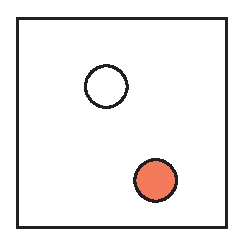
\includegraphics[width=1.5in]{sample.eps}
%  \caption{Lookit! Lookit!}
%}

%% Abstract section.
\abstract{Duis autem vel eum iriure dolor in hendrerit in vulputate
velit esse molestie consequat, vel illum dolore eu feugiat nulla
facilisis at vero eros et accumsan et iusto odio dignissim qui blandit
praesent luptatum zzril delenit augue duis dolore te feugait nulla
facilisi. Lorem ipsum dolor sit amet, consectetuer adipiscing elit,
sed diam nonummy nibh euismod tincidunt ut laoreet dolore magna
aliquam erat volutpat. Ut wisi enim ad minim veniam, quis nostrud exerci tation ullamcorper
suscipit lobortis nisl ut aliquip ex ea commodo consequat. Duis autem
vel eum iriure dolor in hendrerit in vulputate velit esse molestie
consequat, vel illum dolore eu feugiat nulla facilisis at vero eros et
accumsan et iusto odio dignissim qui blandit praesent luptatum zzril
delenit augue duis dolore te feugait nulla facilisi.%
} % end of abstract

%% ACM Computing Classification System (CCS). 
%% See <http://www.acm.org/about/class> for details.
%% We recommend the 2012 system <http://www.acm.org/about/class/class/2012>
%% For the 2012 system use the ``\CCScatTwelve'' which command takes four arguments.
%% The 1998 system <http://www.acm.org/about/class/class/2012> is still possible
%% For the 1998 system use the ``\CCScat'' which command takes four arguments.
%% In both cases the last two arguments (1998) or last three (2012) can be empty.

\CCScatlist{
  \CCScatTwelve{Human-centered computing}{Visu\-al\-iza\-tion}{Visu\-al\-iza\-tion techniques}{Treemaps};
  \CCScatTwelve{Human-centered computing}{Visu\-al\-iza\-tion}{Visualization design and evaluation methods}{}
}

%\CCScatlist{
  %\CCScat{H.5.2}{User Interfaces}{User Interfaces}{Graphical user interfaces (GUI)}{};
  %\CCScat{H.5.m}{Information Interfaces and Presentation}{Miscellaneous}{}{}
%}

%% Copyright space is enabled by default as required by guidelines.
%% It is disabled by the 'review' option or via the following command:
% \nocopyrightspace

%%%%%%%%%%%%%%%%%%%%%%%%%%%%%%%%%%%%%%%%%%%%%%%%%%%%%%%%%%%%%%%%
%%%%%%%%%%%%%%%%%%%%%% START OF THE PAPER %%%%%%%%%%%%%%%%%%%%%%
%%%%%%%%%%%%%%%%%%%%%%%%%%%%%%%%%%%%%%%%%%%%%%%%%%%%%%%%%%%%%%%%%

\begin{document}

%% The ``\maketitle'' command must be the first command after the
%% ``\begin{document}'' command. It prepares and prints the title block.

%% the only exception to this rule is the \firstsection command
\firstsection{Introduction}

\maketitle

%% \section{Introduction} %for journal use above \firstsection{..} instead

%% Importance Of The Area

Virtual Reality and Augmented Reality is about trick our senses to improve our feeling of presence. Several factors influence directly in how successful the user experience is, among them the quality of the rendering, textures and 3D models. But this static part by itself does not produce a fully immersive experience. The behavior of the elements on the environment, the way as they move and how the user interacts with them, play a fundamental role. There are several ways to model the User-environment interaction in immersive environments and its common not to be physical-accurate to reduce computation times or simplify a task that would be harder under real conditions. In this way, a kinematic behavior is quite popular, but if we want to go ahead developing virtual worlds, it becomes necessary to bring the real manner of see and interact with objects. An excellent application to exemplify that development trend is the immersive design or modeling. Virtual modeling is an area becoming greater due to the development of new technologies. This area is promising in the sense that could decrease the time of construction of virtual models or animations. With those technologies, the 3D artists can create artworks that were impossible, or at least very arduous to develop with the classic input methods.\\
 
%% Approaches that existed Before
There are some popular applications used to make 3D creations using immersive interaction, like TiltBrush \cite{TiltBrush} released in 2016 by Google. This application adequately addresses most of the immersive interaction issues when painting in 3d. In the same way, Quill \cite{Quill} by Facebook Let the user not just create virtual models but also animate them. These approaches were successful in letting users materialize ideas, by introducing tools to sculpt, draw, paint. In the case of Quill, adding a timeline to animate frame per frame the scene. Within this paradigm, the user can use some presets to generate animations or create the scene and then animate them.\\

%% Why They Were not satisfactory?
The more noticeable weakness on those tools is the fact of lack of materials, some of the applications indeed, let the user choose a material to create their models, but this is limited just to the rendering. The material behavior is in most of the cases the same than the other materials but with different colors, or different normal map, or different transparency, but in its core remains the same. Also, a lack of physics-based behavior is noticeable: the drawings or the objects created are static and keeps static along the experience. The interaction among objects is entirely kinematic; this dramatically decreases the possibility of creating real-world animations. This choose happens mainly because of the computational cost that a physical model will introduce in the whole applications. Programmers Generally give priority to stability and interactivity with the interface. Currently, literature offers some well-developed methods to simulate this physic behavior. A good cost-effective option is to use position-based simulations because it significantly reduces the computation time of physical-based simulations. Recent developments in this area let us simulate the significant natural phenomena.\\

%% Why ours is better?
Taking into account the issues mentioned above. We propose an immersive sketching application able to create objects with different materials and introducing physical-based interactions between objects in real-time using position-based dynamics (PBD). Making possible the creation of complex animations involving several types of physics behaviors like solids, liquids, gases, deformable and clothes. Our model is unconditionally stable as we optimize position constraints instead of integrating the next positions of the bodies. This approach could be easily extended to simulate more complex physical-based phenomena in immersive sketching but also other immersive applications.\\

%% Reminder
This paper is organized as follows. In section 2. we explore different applications addressing the main components of our method, then in section 3., we present the core concepts of our application and the main techniques implemented, as interaction analogies, animation calculations, particle management, and the virtual tools introduced. After we show the results get with our implementation, and finally we conclude about the relevant aspects of this new approach.


\section{Related Works}

Technologies as virtual reality and computer graphics are growing significantly; those technologies bring new paradigms to the professional and amateur artist. In this section we review the main topics related to our technique:

\subsection{Immersive Design}
Recently some works have proposed the use of immersive methods to let artist sketch, draw and even sculpt. Two must-know applications are Tilt Brush by Google \cite{TiltBrush} and Quill by Facebook \cite{Quill}, both of them was brought a new paradigm when making art. GravitySketch \cite{GravitySketch}, a more recent application also gives an immersive experience and additionally let the user interact without controllers by using leap motion. Works as Canvox by Kim et al. (2017) \cite{Kim2017} and Multiplanes by Barrera et al. (2018) \cite{BarreraMachuca2017} focuses on how the artist does the designs, the first one proposes the division of the whole canvas in smaller volumes of interest to give more details when drawing. In contrast, Multiplanes aid the user to sketch by automatically generating planes as the user draws a line. Seo et al. \cite{Seo2018} presented Aura Garden in 2018, a collaborative sculpting environment for light. This environment lets users draw and animate in mid-air with different materials, but all those materials are non-physical (excluding wood), so it is not possible to simulate interactions among them and with the user. Another Collaborative application in VR is Ontlus by Chen et al. (2018) \cite{Chen2018} where the users can paint and sculpt in the virtual environment. A common failure of those applications is the few or even inexistent physical-based animation on the process, limiting the dynamism of the creations. In this way, the interactivity of the objects decreases.

\subsection{Particle-based Simulations}
 
Lagrangian models are widely used to perform real-time simulations. Methodologies as Position-based dynamics (PBD) \cite{Muller2007} or Smoothed-particle hydrodynamics has become more and more popular lately. Some works were intended to model physical behaviors as solids, fluids \cite{Macklin2013}, gases \cite{ren2016fast} and even complex phenomena as magnetic fields \cite{dolag1999sph} or phase transitions \cite{salazar2018heat}. The main applications of those methods are animation and films, but some works use them in interactive simulations: Pan et al. \cite{Pan2015real} simulated real-time soft tissue cutting with position based dynamics getting very plausible results, after this Berndt et al. \cite{berndt2017efficient} introduced a faster simulation model. An interesting feature of both works is the use of force feedback, that requires even stringent computation times. Despite its capacity of real-time simulation, particle-based methods are mainly used to create animations or movies, and there are few works reporting interactive applications.

\subsection{Physic-based interaction}

Real-time VR physical interactions are not very common in literature, and it makes sense if we think on the complexity of those calculations \cite{Holl2018}. Physical behavior usually implies integration approaches and, despite the current improved integration methods, the timestep is yet a limitation to get simulations working. Generally, its needed to sacrifice one: stability or real-time rates. Kim et al. presented several works around physical-based interaction \cite{Nasim2018, Kim2015, Nasim2016, Kim2016}. They highlight the problems caused because of the mismatch between the real hand and the virtual hand model, their solution is to center the calculations on the object coordinates, but as it remains needing an integration scheme in some form, it is not exempt of instabilities. Position-based approaches have been proven to avoid these problems and allow higher timesteps \cite{Macklin2014}.
Another point to highlight on those works is the use of stereo cameras (LeapMotion) to track the hand. Using that tracking system could lead to abrupt changes in position and somehow restrict the interactive workspace. As we don't use Leap-motion based interactions so, our workspace is bigger and corresponds to the room free space, it constraint us to use other methods to track hands movement as VICON tracking or the HMD controllers, for our implementation we used the last option. The above-cited works also ignore the simulation of rigid bodies or more complex behaviors like clothes.

\section{Methods}

In this section we discuss the main concept needed to understand how our approach is supported.

\subsection{Particle-based Dynamics}

Lagrangian models in contrast with Eulerian approaches, treat the bodies as the origin of its calculations, givin the properties and states to each particle making unnecessary to calculate properties inside a grid, this is useful specially when the domain of the simulation is unknown. There are several meshless methods used to model continuum mechanics, we chosen Position-Based Dynamics \cite{Muller2007} because its unconditionally stability and its low computational cost.
PBD is a particle-based animation technique that uses a set of constraints to calculate the positions of the particles in each timestep. It tries to fit the position of each particle inside the space, based on the available constrains on the particles. A particle can have an arbitrary number of constrains, but a constraint must have at least two particles. As the solver must iterate to set the positions of the particles based in the constraint available space and trying to satisfy each constraint, we can see this as an optimization problem. This is a successful way to simulate a wide variety of bodies like cloths, deformable, rods, elastics but is not capable to simulate by itself fluid volumes or totally rigid bodies
\subsection{Parallel solvers}
\subsection{Voxelization}
\subsection{Particle Management}
\subsubsection{Solids}
\subsubsection{Liquids}
\subsubsection{Gases}
\subsection{Modeling tools}
\subsection{Interaction with objects}
\section{Results}
\section{Conclusion}

A fully immersive experience needs haptic feedback, force feedback or technologies as mid-air haptics. This could improve the performance of digital artists when sculpting or modeling they artwork.



%% if specified like this the section will be committed in review mode
\acknowledgments{
The authors wish to thank A, B, and C. This work was supported in part by
a grant from XYZ.}

%\bibliographystyle{abbrv}
\bibliographystyle{abbrv-doi}
%\bibliographystyle{abbrv-doi-narrow}
%\bibliographystyle{abbrv-doi-hyperref}
%\bibliographystyle{abbrv-doi-hyperref-narrow}

\bibliography{template}
\end{document}
